\documentclass{report}
\usepackage{graphicx} % Required for \includegraphics
\usepackage{float}    % Required for [H] specifier

\begin{document}
\title{Labwork 3: Report}
\author{Nguyen Nhat Anh} % Required by the report class for \maketitle
\maketitle

\section{Introduction}
I have made the image RGB-to-gray converter using Numba CUDA, all the code given are following strictly from report. 

\section{Results}
For CPU:
\begin{figure}[H]
    \centering 
    \includegraphics[width=0.7\linewidth]{cpu_output.jpg}
    \caption{CPU image output.}
    \label{fig:cpu_image} 
\end{figure}

For GPU:
\begin{figure}[H]
    \centering 
    \includegraphics[width=0.7\linewidth]{output_gpu.jpg}
    \caption{GPU image output.}
    \label{fig:gpu_image}
\end{figure}

Runtime:
\begin{figure}[H]
    \centering 
    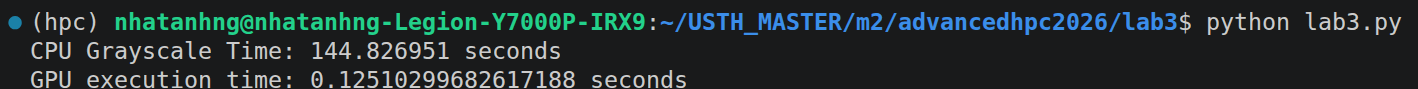
\includegraphics[width=0.7\linewidth]{runtime.png}
    \caption{Runtime comparison between CPU and GPU.}
    \label{fig:runtime_image}
\end{figure}

\section{Discussion}
The results show that the GPU implementation significantly outperforms the CPU implementation in terms of runtime. The GPU implementation is more efficient for image conversion.

\end{document}